%%!TEX root = main.Rnw
%\documentclass[english, 11pt]{article}
%\usepackage{haziq_article}
%\begin{document}



For the purposes of this section, we shall be looking at the \code{MASS::cats} data set, which contains $n = 144$ samples of body weights of male and female cats, from which we would like to predict their corresponding heart weights.

\begin{knitrout}
\definecolor{shadecolor}{rgb}{1, 1, 1}\color{fgcolor}\begin{kframe}
\begin{alltt}
\hlkwd{data}\hlstd{(cats,} \hlkwc{package} \hlstd{=} \hlstr{"MASS"}\hlstd{);} \hlkwd{str}\hlstd{(cats)}
\end{alltt}
\begin{verbatim}
## 'data.frame':	144 obs. of  3 variables:
##  $ Sex: Factor w/ 2 levels "F","M": 1 1 1 1 1 1 1 1 1 1 ...
##  $ Bwt: num  2 2 2 2.1 2.1 2.1 2.1 2.1 2.1 2.1 ...
##  $ Hwt: num  7 7.4 9.5 7.2 7.3 7.6 8.1 8.2 8.3 8.5 ...
\end{verbatim}
\end{kframe}
\end{knitrout}

The three subsections that follow begins with an introduction to the basic \pkg{iprior} package functionality, and then a discussion on the kernel loader feature and various model and fitting options.

\section{Introduction}\label{sec:ipriorpkgintro}

The \pkg{iprior} package supports both formula and non-formula input. The syntax to perform I-prior modelling which regresses the responses \code{Hwt} on covariates \code{Bwt} and \code{Sex} is as follows:

\begin{knitrout}
\definecolor{shadecolor}{rgb}{1, 1, 1}\color{fgcolor}\begin{kframe}
\begin{alltt}
\hlstd{mod.fit} \hlkwb{<-} \hlkwd{iprior}\hlstd{(Hwt} \hlopt{~} \hlstd{Bwt} \hlopt{+} \hlstd{Sex,} \hlkwc{data} \hlstd{= cats)}  \hlcom{# formula syntax}
\hlstd{mod.fit} \hlkwb{<-} \hlkwd{iprior}\hlstd{(}\hlkwc{y} \hlstd{= cats}\hlopt{$}\hlstd{Hwt, cats}\hlopt{$}\hlstd{Bwt, cats}\hlopt{$}\hlstd{Sex)}  \hlcom{# non-formula syntax}
\end{alltt}
\end{kframe}
\end{knitrout}


This would fit an I-prior model with two scale parameters, one for each of the two covariates \code{Bwt} and \code{Sex}:
\begin{align*}
\begin{gathered}
  \texttt{Hwt} = \text{intercept} + \mathbf H_\lambda\mathbf w + \bepsilon \\
  \bepsilon \sim \N(\bzero, \psi^{-1}\mathbf I_n) \\
  \mathbf w \sim \N(\bzero, \psi\bI_n) \\
  \bH_\lambda = \lambda_1 H(\texttt{Bwt}) + \lambda_2 H(\texttt{Sex}).
\end{gathered}
\end{align*}

We have used the notation $H(\texttt{x})$ to denote the kernel matrix for the covariate \code{x}, i.e., $H(\texttt{x})$ is a $n \times n$ symmetric matrix whose $(i,j)$th entry is $h(\texttt{x[i]}, \texttt{x[j]})$, with $h$ being one of the canonical, FBM or Pearson kernel functions. The object \code{x} can either be a vector of length $n$, or a $n \times c$ matrix representing a (functional) covariate. Out of interest, the three kernel matrices are exposed in the \pkg{iprior} package as \texttt{fnH2()}, \texttt{fnH3()} and \texttt{fnH1()} respectively. Incidentally, $\lambda_1$ and $\lambda_2$ are the scale parameters to be estimated, along with the error precision $\psi$.

The two lines of code shown earlier are equivalent ways of fitting the same I-prior model. In the formula syntax, the first argument is the \code{formula} of the I-prior model, which is the familiar base \proglang{R} symbolic description of models, and the second argument is the data frame containing the variables in the model formula. In the non-formula syntax, the first argument is the response variable \code{y}, and this is followed by as many explanatory variables as required, separated by commas. Unlike in the formula syntax, the non-formula syntax allows these explanatory variables to be matrices, where each matrix would represent a single multi-dimensional covariate.

The resulting object \code{mod.fit} is an S3 object of class \code{ipriorMod}. Similar to a linear model object of class \code{lm}, several methods were either specially coded or is compatible with the default \proglang{R} methods. The methods which are available are listed in Table \ref{tab:methods} below. The object \code{mod.fit} also contains other items pertinent to an I-prior model which the user can extract manually via list indexing, such as the posterior means of the random effects, $\hat w_1, \dots, \hat w_n$ (\code{mod.fit\$w.hat}) and the number of EM iterations performed (\code{mod.fit\$no.iter}).

\begin{table}[h]
\centering
\begin{tabular}{lp{10cm}}
\hline
\proglang{R} Function & Description \\
\hline
\code{coef}     & Extracts the estimates of the parameters (intercept, scale parameters and error precision) of the I-prior model. \\
\Top
\code{sigma}    & Extracts the estimate of the model standard deviation of errors (i.e., square root of the inverse error precision). \\
\Top
\code{fitted}   & Returns the fitted value of the responses $\hat y_1, \dots, \hat y_n$. \\
\Top
\code{predict}  & Calculates fitted values from a new set of covariates. \\
\Top
\code{resid}    & Returns the residuals $\hat\varepsilon_1, \dots, \hat\varepsilon_n$. \\
\code{plot}     & Produces three kinds of plots: 1) Plot of the fitted regression curve, 2) Plot of fitted values against residuals, and 3) a Normal Q-Q plot of the residuals.  \\
\Top
\code{logLik}   & Returns the log-likelihood value of the fitted I-prior model at the ML estimates, or at a user-input set of parameters \code{theta = c(lambda, psi)}. \\
\Top
\code{deviance} & Returns twice the negative log-likelihood value. \\
\Top
\code{Hlam} & Extracts the scaled kernel matrix, $\mathbf H_\lambda$. \\
\Top
\code{vary} & Calculates the variance of $y$, $\mathbf V_y$.\\
\hline
\end{tabular}
\caption{Available methods for an object of class \code{ipriorMod}.}
\label{tab:methods}
\end{table}

An \code{ipriorMod} object summary reveals the model call, the RKHS and scale parameters used on the covariates, the five-number summary of the residuals, and the parameter estimates along with their standard errors and the corresponding tests of nullity. The mathematical details on how these were obtained can be found in the appendix. The summary also contains information on the EM algorithm convergence and the final log-likelihood value attained. By design, the summary was intended to look similar to an \code{lm} object summary.

\begin{knitrout}
\definecolor{shadecolor}{rgb}{1, 1, 1}\color{fgcolor}\begin{kframe}
\begin{alltt}
\hlkwd{summary}\hlstd{(mod.fit)}
\end{alltt}
\begin{verbatim}
## 
## Call:
## iprior(formula = Hwt ~ Bwt + Sex, data = cats)
## 
## RKHS used:
## Pearson (Sex) 
## Canonical (Bwt) 
## with multiple scale parameters.
## 
## Residuals:
##     Min.  1st Qu.   Median  3rd Qu.     Max. 
## -3.55800 -0.95300 -0.08797  1.05200  5.13600 
## 
##             Estimate    S.E.      z P[|Z>z|]    
## (Intercept)  10.6306  0.1206 88.150   <2e-16 ***
## lam1.Bwt      0.9972  0.7022  1.420    0.156    
## lam2.Sex     -0.0025  0.0171 -0.144    0.886    
## ---
## Signif. codes:  0 '***' 0.001 '**' 0.01 '*' 0.05 '.' 0.1 ' ' 1
## 
## EM converged to within 1e-07 tolerance. No. of iterations: 691
## Standard deviation of errors: 1.447 with S.E.: 0.0856
## Log-likelihood value: -260.3357
\end{verbatim}
\end{kframe}
\end{knitrout}

Notice that the canonical kernel was used for \code{Bwt} and the Pearson kernel for factor type object \code{Sex}. As we will see later on, we can specify which kernels we would like to use and also manipulate how the scale parameter(s) come into effect.

\section{Kernel loader and flexible fitting}

Included in the \pkg{iprior} package is the \code{kernL()} function, which allows the data to be ``loaded'' into an \code{ipriorKernel} object. This mainly performs and stores all the necessary matrix multiplications to ready the kernel matrices, which can then be called on later during the fitting procedure. The \code{kernL()} function would also determine the number of scale parameters to use, based on the user's input regarding parsimony, interactions, and higher order terms (see Section \ref{sec:options} for model options). The syntax is exactly the same as the \code{iprior()} function, with both formula and non-formula syntax supported.

\begin{knitrout}
\definecolor{shadecolor}{rgb}{1, 1, 1}\color{fgcolor}\begin{kframe}
\begin{alltt}
\hlstd{mod} \hlkwb{<-} \hlkwd{kernL}\hlstd{(Hwt} \hlopt{~} \hlstd{Bwt} \hlopt{+} \hlstd{Sex,} \hlkwc{data} \hlstd{= cats)}  \hlcom{# formula syntax}
\hlstd{mod} \hlkwb{<-} \hlkwd{kernL}\hlstd{(}\hlkwc{y} \hlstd{= cats}\hlopt{$}\hlstd{Hwt, cats}\hlopt{$}\hlstd{Bwt, cats}\hlopt{$}\hlstd{Sex)}  \hlcom{# non-formula syntax}
\end{alltt}
\end{kframe}
\end{knitrout}


There are two reasons for having a kernel loader function. Firstly, I-prior models can sometimes involve high-dimensional matrix multiplications, and these may take a long time to process. By ``loading the kernel'', the user is able to have a stored \code{ipriorKernel} object which can then be reused. A situation where this would be useful would be when the user would like to restart the EM algorithm from different set of starting values. Rather than having to go through all the kernel loading process all over again, the user can simply call on the saved \code{ipriorKernel} object.

Secondly, the \code{kernL()} function allows for flexibile model fitting. The \code{logLik()} and \code{deviance()} method can be used on an \code{ipriorKernel} object, which then can be fed to an optimizer in order to obtain maximum likelihood estimates directly instead of using the EM algorithm. In some instances, this may be a quicker way to obtain model estimates as the EM algorithm can be slow to converge. However, direct optimization generally does not work well when there are a lot of scale parameters to estimate.

\begin{figure}[hbt]
  \centering
  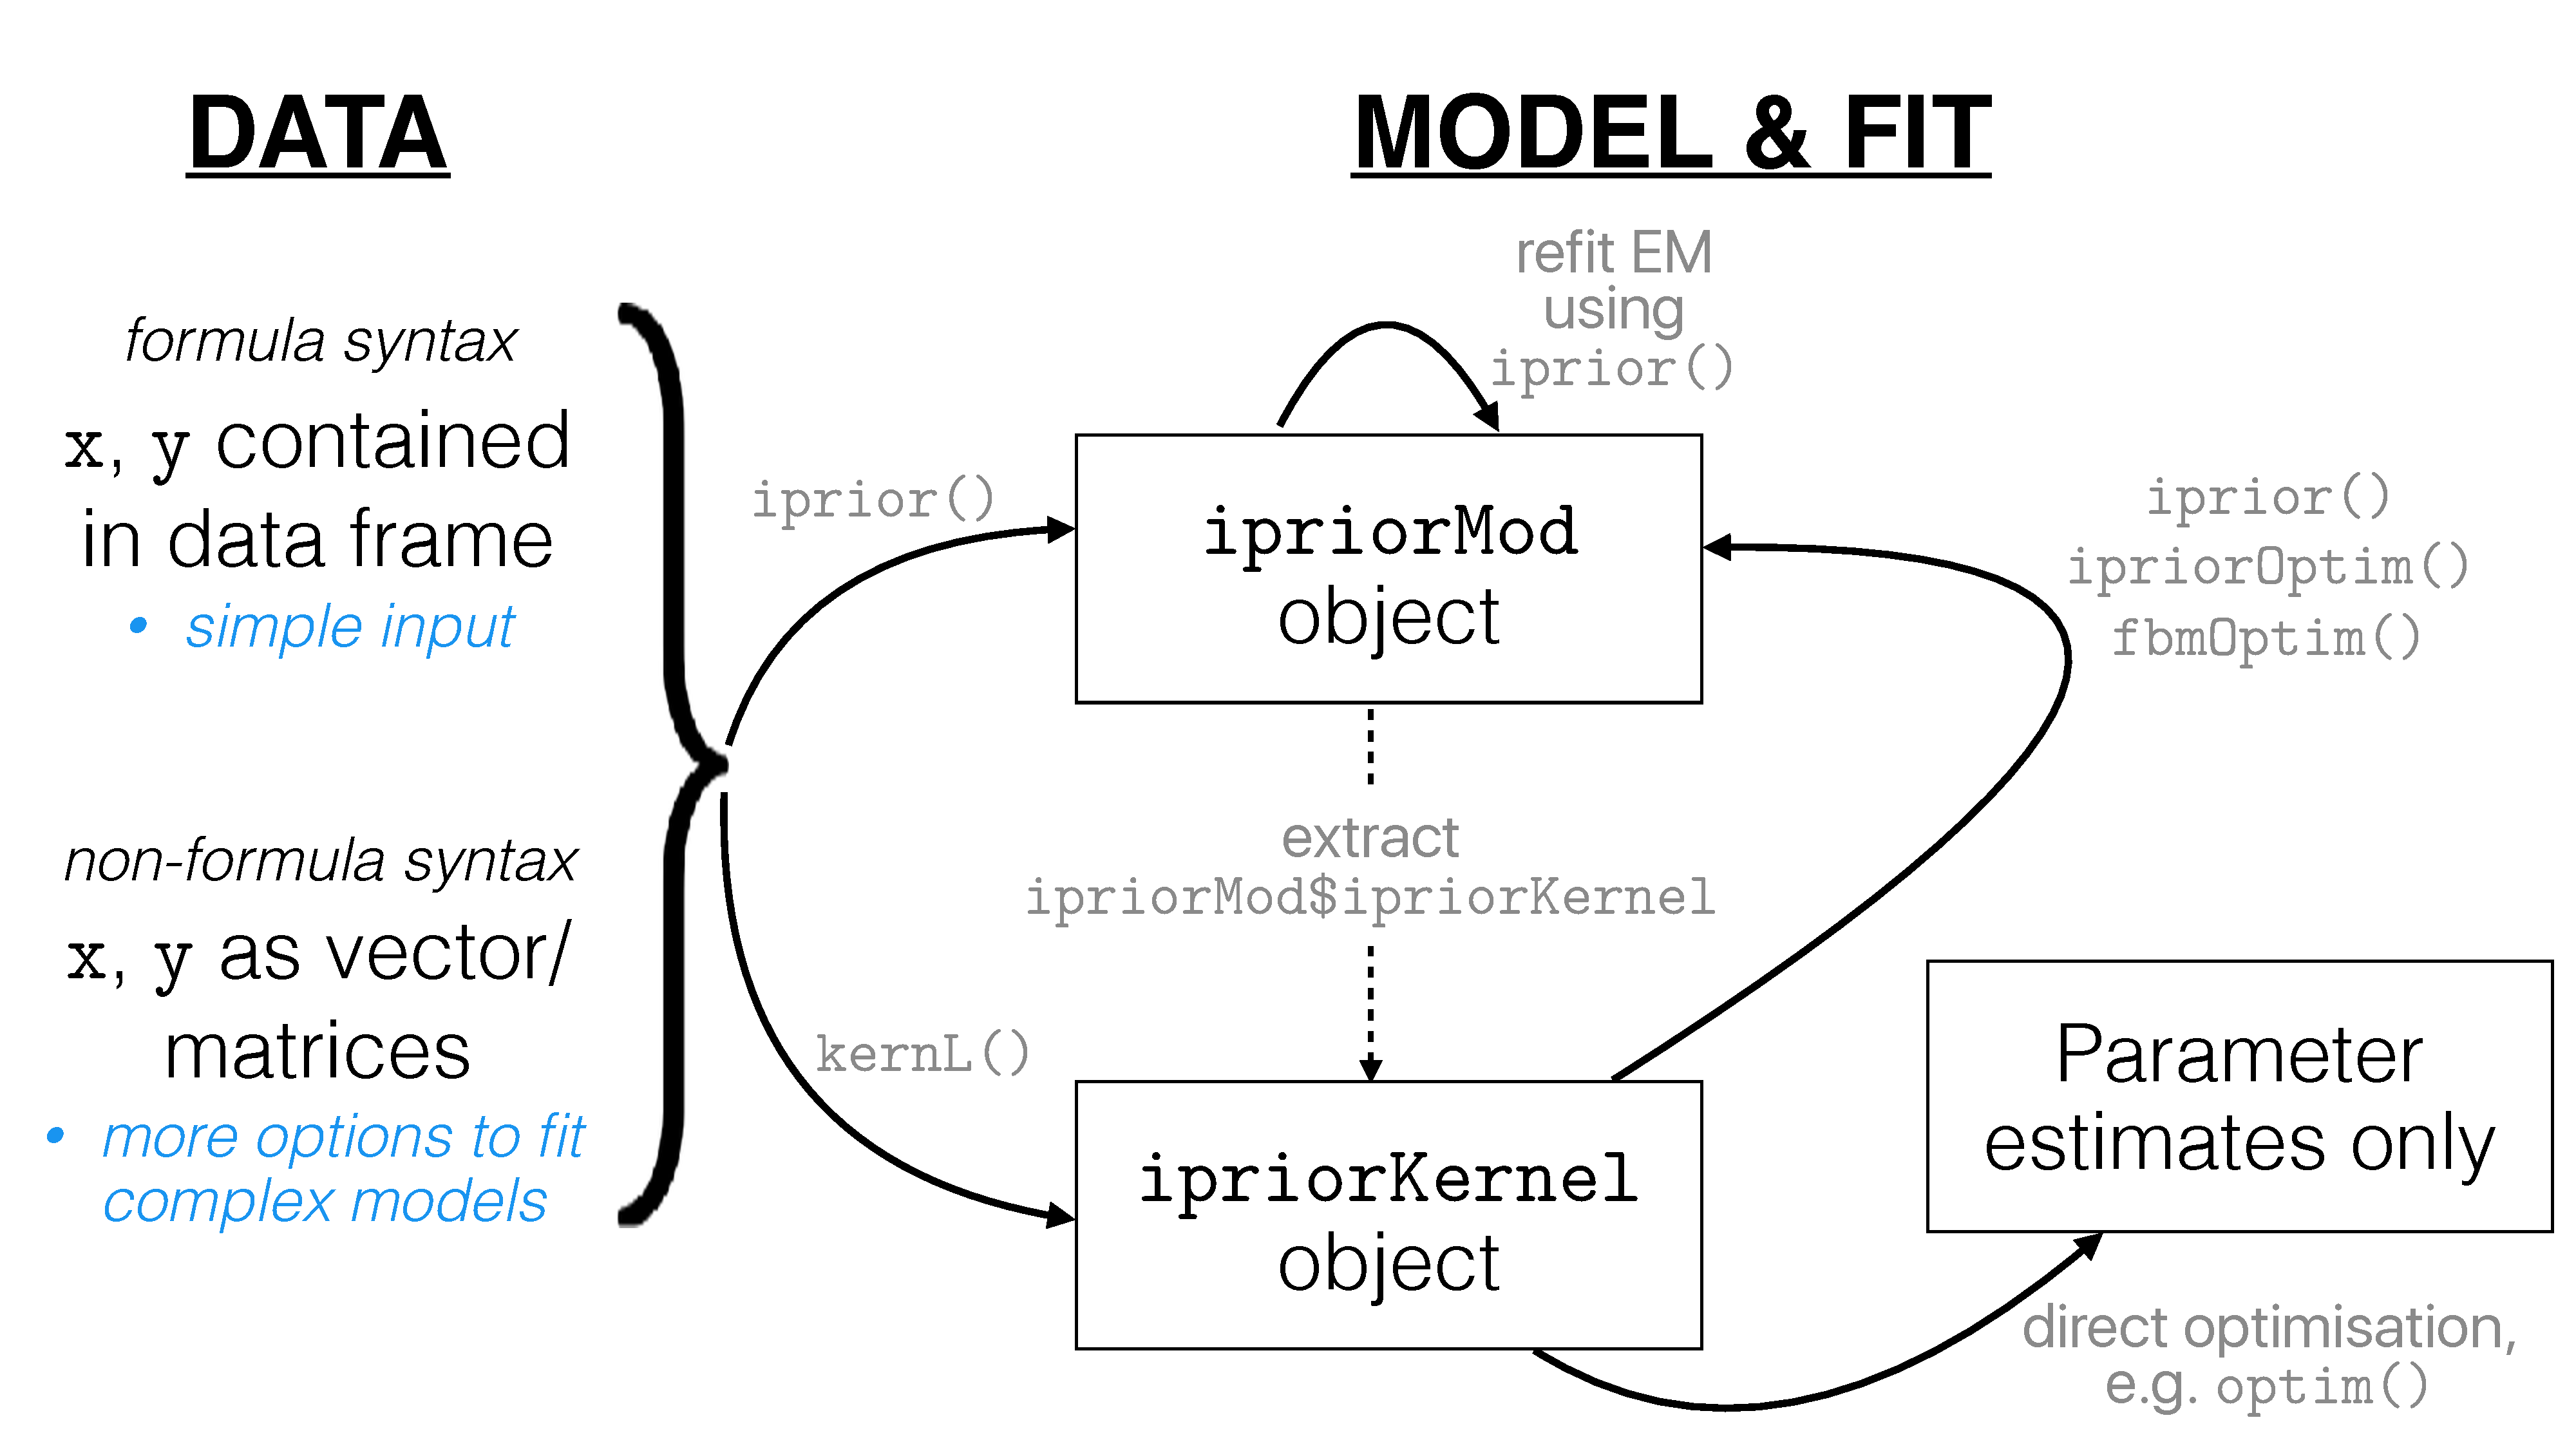
\includegraphics[scale=0.2]{figure/ipriorways.pdf}
  \caption{The different ways of fitting an I-prior model using \code{iprior()}, \code{ipriorKernel}, \code{ipriorOptim()}, \code{fbmOptim()} and even other \proglang{R} optimizers.}
\end{figure}
\label{sec:iprioroptim}
This package also includes a wrapper function called \code{ipriorOptim()} which performs a combination of EM algorithm and direct minimization of the deviance using \proglang{R}'s general-purpose optimization function \code{optim()}. Note that \code{ipriorOptim()} only takes in objects of class \code{ipriorKernel}, so the model has to be specified via the \code{kernL()} function. \code{ipriorOptim()} performs three initial iterations of the EM algorithm, which should be sufficient to get the estimates in the optimal region, and then \code{optim()} takes over to further improve the estimates. The user has control over how many initial EM steps should be performed. The resulting output of this fitting scheme is an object of class \code{ipriorMod}.

The following chunk of code compares how fast it is to fit the \code{cats} data set with interactions three different ways. For direct optimization using \code{optim()}, the \code{par} argument takes the form \code{(lambda[1], ..., lambda[p], psi)}. Note also that we must choose a \code{method} which supports bounds on the parameters - in our case we require the \code{psi} parameter to be greater than zero.

\begin{knitrout}
\definecolor{shadecolor}{rgb}{1, 1, 1}\color{fgcolor}\begin{kframe}
\begin{alltt}
\hlstd{mod} \hlkwb{<-} \hlkwd{kernL}\hlstd{(Hwt} \hlopt{~} \hlstd{Bwt} \hlopt{+} \hlstd{Sex} \hlopt{+} \hlstd{Bwt}\hlopt{:}\hlstd{Sex,} \hlkwc{data} \hlstd{= cats)}
\hlkwd{microbenchmark}\hlstd{(}
  \hlkwc{iprior}      \hlstd{=} \hlkwd{iprior}\hlstd{(mod,} \hlkwc{control} \hlstd{=} \hlkwd{list}\hlstd{(}\hlkwc{silent} \hlstd{=} \hlnum{TRUE}\hlstd{)),}
  \hlkwc{ipriorOptim} \hlstd{=} \hlkwd{ipriorOptim}\hlstd{(mod,} \hlkwc{control} \hlstd{=} \hlkwd{list}\hlstd{(}\hlkwc{silent} \hlstd{=} \hlnum{TRUE}\hlstd{)),}
  \hlkwc{optim}       \hlstd{=} \hlkwd{optim}\hlstd{(}\hlkwc{par} \hlstd{=} \hlkwd{abs}\hlstd{(}\hlkwd{rnorm}\hlstd{(}\hlnum{3}\hlstd{)),} \hlkwc{fn} \hlstd{= deviance,} \hlkwc{object} \hlstd{= mod,}
                      \hlkwc{method} \hlstd{=} \hlstr{"L-BFGS-B"}\hlstd{,} \hlkwc{lower} \hlstd{=} \hlkwd{c}\hlstd{(}\hlopt{-}\hlnum{Inf}\hlstd{,} \hlopt{-}\hlnum{Inf}\hlstd{,} \hlnum{1e-9}\hlstd{)),}
\hlkwc{times} \hlstd{=} \hlnum{10L}\hlstd{)}
\end{alltt}
\begin{verbatim}
## Unit: milliseconds
##         expr       min        lq     mean   median       uq      max neval
##       iprior 8247.5569 8446.9092 8749.932 8826.639 8957.664 9183.745    10
##  ipriorOptim  690.1767  932.2227 1026.394 1035.481 1066.248 1470.554    10
##        optim 1115.2286 1307.5528 1480.510 1367.157 1389.906 2837.722    10
##  cld
##    c
##  a  
##   b
\end{verbatim}
\end{kframe}
\end{knitrout}

From the results, direct optimization is often the fastest method, followed closely by \code{ipriorOptim}, while the slowest method is the EM algorithm. As mentioned, for fairly simple models direct optimization may be the fastest method, but the EM algorithm is more stable when there are a lot of \code{lambda} parameters to be estimated. A combination of both methods via \code{ipriorOptim} may be ideal.

If a model with the FBM kernel is being fitted, one can attempt to find the Hurst coefficient which maximizes the likelihood of the I-prior model. To do this, perform an interval search in $[0,1]$ to minimize the profiled deviance, $D(\gamma) = -2 \log f(\mathbf y; \gamma, \blambda(\gamma), \psi(\gamma))$. This is possible with \pkg{iprior}'s \code{fbmOptim()} function, which makes use of \proglang{R}'s base \code{optimize()} function. Improvements in log-likelihood value can indeed be achieved using this method, and an example of this is shown in Section \ref{sec:tecator}.

\section{Options}
\label{sec:options}

There are two kinds of options (which are input as lists) - one for model control called \code{model}, and one for fitting control called \code{control}. Model options apply to both \code{iprior()} and \code{kernL()} functions, but control options apply only to \code{iprior()} as it is basically specifying control over the EM algorithm. The user sets the options using the syntax
\begin{center}
\code{iprior(formula, data, model = list(...), control = list(...))}.
\end{center}
% <<syntax.options, eval = FALSE>>=
% iprior(formula, data, model = list(...), control = list(...))
% @
The available \code{model} and \code{control} options are explained in the following subsections.

\subsection{Model options}

Model options allow fitting of complex I-prior models. Note that in what follows, the models are purely for illustration of the \code{model} options only, and are not necessarily based on any particular modelling rationale. The argument \code{model}, which is called with \code{iprior()} or \code{kernL()}, is a list of the following items:

\begin{enumerate}

\item \code{kernel}

This allows specification of the type of RKHS used for each continuous covariate. Available choices are \code{"Canonical"}, \code{"FBM"} or \code{"Pearson"}. By default, the canonical kernel is used for continuous variables, and note that the Pearson kernel is always used for factor-type variables. If the user wishes to use either the canonical or FBM kernel instead then some pre-processing must be done to the data beforehand to ``unfactorise'' the variable.

In the \code{MASS::cats} example, the canonical kernel was used for the \code{Bwt} variable. To use the FBM kernel instead, the syntax is as follows:

\begin{knitrout}
\definecolor{shadecolor}{rgb}{1, 1, 1}\color{fgcolor}\begin{kframe}
\begin{alltt}
\hlstd{mod.fit} \hlkwb{<-} \hlkwd{iprior}\hlstd{(Hwt} \hlopt{~} \hlstd{Bwt} \hlopt{+} \hlstd{Sex,} \hlkwc{data} \hlstd{= cats,}
                  \hlkwc{model} \hlstd{=} \hlkwd{list}\hlstd{(}\hlkwc{kernel} \hlstd{=} \hlstr{"FBM"}\hlstd{))}
\end{alltt}
\end{kframe}
\end{knitrout}

One can also specify different kernels for different variables, such as:

\begin{knitrout}
\definecolor{shadecolor}{rgb}{1, 1, 1}\color{fgcolor}\begin{kframe}
\begin{alltt}
\hlstd{mod.fit} \hlkwb{<-} \hlkwd{iprior}\hlstd{(Hwt} \hlopt{~} \hlstd{Bwt} \hlopt{+} \hlkwd{I}\hlstd{(Bwt}\hlopt{^}\hlnum{2}\hlstd{)} \hlopt{+} \hlkwd{I}\hlstd{(Bwt}\hlopt{^}\hlnum{3}\hlstd{),} \hlkwc{data} \hlstd{= cats,}
                  \hlkwc{model} \hlstd{=} \hlkwd{list}\hlstd{(}\hlkwc{kernel} \hlstd{=} \hlkwd{c}\hlstd{(}\hlstr{"FBM"}\hlstd{,} \hlstr{"Canonical"}\hlstd{,} \hlstr{"FBM"}\hlstd{)))}
\end{alltt}
\end{kframe}
\end{knitrout}

In the above example, \code{Hwt} is regressed against \code{Bwt}, \code{Bwt} squared and \code{Bwt} cubed using the kernels FBM, canonical and FBM respectively on the three covariates. To explicitly specify the Hurst coefficient, use the syntax \code{"FBM,<value>"}; otherwise the default of 0.5 is used. As an example, to set the Hurst coefficient equal to 0.1 and 0.2 for the two FBM kernels in the earlier example, the command is as follows:

\begin{knitrout}
\definecolor{shadecolor}{rgb}{1, 1, 1}\color{fgcolor}\begin{kframe}
\begin{alltt}
\hlstd{mod.fit} \hlkwb{<-} \hlkwd{iprior}\hlstd{(Hwt} \hlopt{~} \hlstd{Bwt} \hlopt{+} \hlkwd{I}\hlstd{(Bwt}\hlopt{^}\hlnum{2}\hlstd{)} \hlopt{+} \hlkwd{I}\hlstd{(Bwt}\hlopt{^}\hlnum{3}\hlstd{),} \hlkwc{data} \hlstd{= cats,}
                  \hlkwc{model} \hlstd{=} \hlkwd{list}\hlstd{(}\hlkwc{kernel} \hlstd{=} \hlkwd{c}\hlstd{(}\hlstr{"FBM,0.1"}\hlstd{,} \hlstr{"Canonical"}\hlstd{,}
                                          \hlstr{"FBM,0.2"}\hlstd{)))}
\end{alltt}
\end{kframe}
\end{knitrout}

When multiple regressors are present and we wish to use an FBM kernel with (or without) a user-defined Hurst value, it is sufficient to simply specify the kernel once:

\begin{knitrout}
\definecolor{shadecolor}{rgb}{1, 1, 1}\color{fgcolor}\begin{kframe}
\begin{alltt}
\hlstd{mod.fit} \hlkwb{<-} \hlkwd{iprior}\hlstd{(Hwt} \hlopt{~} \hlstd{Bwt} \hlopt{+} \hlkwd{I}\hlstd{(Bwt}\hlopt{^}\hlnum{2}\hlstd{)} \hlopt{+} \hlkwd{I}\hlstd{(Bwt}\hlopt{^}\hlnum{3}\hlstd{),} \hlkwc{data} \hlstd{= cats,}
                  \hlkwc{model} \hlstd{=} \hlkwd{list}\hlstd{(}\hlkwc{kernel} \hlstd{=} \hlstr{"FBM,0.3"}\hlstd{))}
\end{alltt}
\end{kframe}
\end{knitrout}

This then sets the FBM kernel with Hurst coefficient 0.3 to all of the three regressors.

% \item \code{Hurst}
%
% It is also possible to set the value of the Hurst coefficient for all the Fractional Brownian Motion kernels used, rather than one by one. It is a numeric value between 0 and 1, and defaults to 0.5. This is only applicable when the FBM kernel is used. The following commands are equivalent:
%
% <<syntax.kernel4, eval = FALSE>>=
% kernL(Hwt ~ Bwt + I(Bwt^2) + I(Bwt^3), data = cats,
%       model = list(kernel = "FBM,0.1"))
% kernL(Hwt ~ Bwt + I(Bwt^2) + I(Bwt^3), data = cats,
%       model = list(kernel = "FBM", Hurst = 0.1))
% @
%
% Note that if the syntax `kernel = "FBM,<value1>"` is used together with the option `Hurst = <value2>`, then the `Hurst` option overrides the individual Hurst specification.

\item \code{parsm}

A logical vector which defaults to \code{TRUE} to indicate whether parsimonious interactions should be used or not. When interactions are present in an I-prior model, there are two ways to handle the scale parameters of the kernels: the parsimonious method and the non-parsimonious method. The code below demonstrates the \code{parsm} option using the package's kernel loader function on the \code{cats} data set.

\begin{knitrout}
\definecolor{shadecolor}{rgb}{1, 1, 1}\color{fgcolor}\begin{kframe}
\begin{alltt}
\hlcom{# parsm = TRUE (by default)}
\hlstd{(mod} \hlkwb{<-} \hlkwd{kernL}\hlstd{(Hwt} \hlopt{~} \hlstd{Bwt} \hlopt{+} \hlstd{Sex} \hlopt{+} \hlstd{Bwt}\hlopt{:}\hlstd{Sex,} \hlkwc{data} \hlstd{= cats))}
\end{alltt}
\end{kframe}
\end{knitrout}
\begin{knitrout}
\definecolor{shadecolor}{rgb}{1, 1, 1}\color{fgcolor}\begin{kframe}
\begin{verbatim}
## 
## Sample size =  144 
## Number of x variables, p =  2 
## Number of scale parameters, l =  2 
## Number of interactions =  1 
## 
## Info on H matrix:
## 
## List of 3
##  $ Bwt    : Canonical [1:144, 1:144] 0.524 0.524 0.524 0.451 0.451 ...
##  $ Sex    : Pearson [1:144, 1:144] 2.06 2.06 2.06 2.06 2.06 ...
##  $ Bwt:Sex: Canonical x Pearson [1:144, 1:144] 1.081 1.081 1.081 0.9..
\end{verbatim}
\end{kframe}
\end{knitrout}
\begin{knitrout}
\definecolor{shadecolor}{rgb}{1, 1, 1}\color{fgcolor}\begin{kframe}
\begin{alltt}
\hlcom{# compare with parsm = FALSE}
\hlstd{(mod} \hlkwb{<-} \hlkwd{kernL}\hlstd{(Hwt} \hlopt{~} \hlstd{Bwt} \hlopt{+} \hlstd{Sex} \hlopt{+} \hlstd{Bwt}\hlopt{:}\hlstd{Sex,} \hlkwc{data} \hlstd{= cats,}
              \hlkwc{model} \hlstd{=} \hlkwd{list}\hlstd{(}\hlkwc{parsm} \hlstd{=} \hlnum{FALSE}\hlstd{)))}
\end{alltt}
\end{kframe}
\end{knitrout}
\begin{knitrout}
\definecolor{shadecolor}{rgb}{1, 1, 1}\color{fgcolor}\begin{kframe}
\begin{verbatim}
## 
## Sample size =  144 
## Number of x variables, p =  2 
## Number of scale parameters, l =  3 
## Number of interactions =  1 
## 
## Info on H matrix:
## 
## List of 3
##  $ Bwt    : Canonical [1:144, 1:144] 0.524 0.524 0.524 0.451 0.451 ...
##  $ Sex    : Pearson [1:144, 1:144] 2.06 2.06 2.06 2.06 2.06 ...
##  $ Bwt:Sex: Canonical x Pearson [1:144, 1:144] 1.081 1.081 1.081 0.9..
\end{verbatim}
\end{kframe}
\end{knitrout}
The kernel matrices produced would be exactly the same, except that in the parsimonious case, there are only two scale parameters (one for each covariate), while in the non-parsimonious case, there is an additional scale parameter added for the interaction term. Roughly speaking, the difference between the two methods is illustrated by the two formulae\footnotemark

\begin{align*}
  \text{parsimonious } &: \mathbf H_\lambda  = \lambda_1 H(\texttt{Bwt}) + \lambda_2 H(\texttt{Sex}) + \lambda_1 \lambda_2 \ H(\texttt{Bwt}) \circ H(\texttt{Sex}) \\
  \text{non-parsimonious } &: \mathbf H_\lambda  = \lambda_1 H(\texttt{Bwt}) + \lambda_2 H(\texttt{Sex}) + \hspace{4mm} \lambda_3 \ H(\texttt{Bwt}) \circ H(\texttt{Sex}).
\end{align*}

\footnotetext{$\circ$ is the Hadamard entrywise product for matrices of the same dimensions.}
% where $h(\texttt{x})$ is the kernel function applied to the variable \code{x}.

\item \code{order}

This option is related to the parsimony option, in that it lets the \code{iprior()} or \code{kernL()} function know whether or not any of the variables have been raised to a higher power. If so, the scale parameter for the higher order variable would be the scale parameter of the original variable raised to the same power. If this is not specified, then a separate scale parameter is used.

\code{order} is a character vector of length equal to the number of covariates. The syntax is \verb@"a^b"@, to indicate that the covariate at position \code{a} raised is to the power \code{b}. For any variable not raised to a power, simply put \code{a}. In the following example, only one scale parameter is used because the three covariates in the model make up a polynomial (of order 3 in this case).

\begin{knitrout}
\definecolor{shadecolor}{rgb}{1, 1, 1}\color{fgcolor}\begin{kframe}
\begin{alltt}
\hlstd{(mod} \hlkwb{<-} \hlkwd{kernL}\hlstd{(Hwt} \hlopt{~} \hlstd{Bwt} \hlopt{+} \hlkwd{I}\hlstd{(Bwt}\hlopt{^}\hlnum{2}\hlstd{)} \hlopt{+} \hlkwd{I}\hlstd{(Bwt}\hlopt{^}\hlnum{3}\hlstd{),} \hlkwc{data} \hlstd{= cats,}
              \hlkwc{model} \hlstd{=} \hlkwd{list}\hlstd{(}\hlkwc{order} \hlstd{=} \hlkwd{c}\hlstd{(}\hlstr{"1"}\hlstd{,} \hlstr{"1^2"}\hlstd{,} \hlstr{"1^3"}\hlstd{))))}
\end{alltt}
\begin{verbatim}
## 
## Sample size =  144 
## Number of x variables, p =  3 
## Number of scale parameters, l =  1 
## Number of interactions =  0 
## 
## Info on H matrix:
## 
## List of 3
##  $ Bwt     : Canonical [1:144, 1:144] 0.524 0.524 0.524 0.451 0.451 ...
##  $ I(Bwt^2): Canonical [1:144, 1:144] 13.3 13.3 13.3 11.8 11.8 ...
##  $ I(Bwt^3): Canonical [1:144, 1:144] 201 201 201 183 183 ...
\end{verbatim}
\end{kframe}
\end{knitrout}

The kernel matrix implied by this model is of course
\[
  \mathbf H_\lambda  = \lambda H(\texttt{Bwt}) + \lambda^2 H(\verb@Bwt^2@) + \lambda^3 H(\verb@Bwt^3@).
\]

\item \code{one.lam}

A logical vector to indicate whether or not a single scale parameter should be used for all covariates. This defaults to \code{FALSE}. This really is only relevant when using formula call, because the model input using non-formula is able to distinguish between using a single or multiple scale parameters. For instance, the two model calls are identical:

\begin{knitrout}
\definecolor{shadecolor}{rgb}{1, 1, 1}\color{fgcolor}\begin{kframe}
\begin{alltt}
\hlcom{# Formula input}
\hlstd{mod.fit} \hlkwb{<-} \hlkwd{iprior}\hlstd{(Hwt} \hlopt{~} \hlstd{Bwt} \hlopt{+} \hlstd{Sex,} \hlkwc{data} \hlstd{= cats,}
                  \hlkwc{model} \hlstd{=} \hlkwd{list}\hlstd{(}\hlkwc{one.lam} \hlstd{=} \hlnum{TRUE}\hlstd{))}
\end{alltt}
\end{kframe}
\end{knitrout}
\begin{knitrout}
\definecolor{shadecolor}{rgb}{1, 1, 1}\color{fgcolor}\begin{kframe}
\begin{alltt}
\hlcom{# Non-formula input}
\hlstd{mod.fit} \hlkwb{<-} \hlkwd{iprior}\hlstd{(}\hlkwc{y} \hlstd{= cats}\hlopt{$}\hlstd{Hwt, cats[,} \hlkwd{c}\hlstd{(}\hlstr{"Bwt"}\hlstd{,} \hlstr{"Sex"}\hlstd{)])}
\end{alltt}
\end{kframe}
\end{knitrout}

The non-formula input treats the objects following the \code{y} argument as individual covariates. In this case, the object \code{cats[, c("Bwt", "Sex")]} is a matrix containing both the \code{Bwt} and \code{Sex} variables, and because it is contained in the matrix as one object, a single scale parameter is used. Note that it is not necessary to use the \code{one.lam} option when using non-formula syntax. With the \code{one.lam = TRUE} option, we are fitting an I-prior model with the following kernel:

\[
  \mathbf H_\lambda = \lambda \left( H(\texttt{Bwt}) + H(\texttt{Sex}) \right).
\]

This option is suitable to be used when all explanatory variables are measured on the same scale, or alternatively, the explanatory variables have been standardised before fitting the model.

\item \code{interactions}

While interactions are automatically dealt with when using formula syntax, this needs to be specified when using non-formula syntax. This is specified using the syntax \code{"a:b"} to indicate that the variable in position \code{a} interacts with the variable in position \code{"b"}. The following two model calls are then identical:

\begin{knitrout}
\definecolor{shadecolor}{rgb}{1, 1, 1}\color{fgcolor}\begin{kframe}
\begin{alltt}
\hlcom{# Formula input}
\hlstd{mod.fit} \hlkwb{<-} \hlkwd{iprior}\hlstd{(Hwt} \hlopt{~} \hlstd{Bwt} \hlopt{+} \hlstd{Sex} \hlopt{+} \hlstd{Bwt}\hlopt{:}\hlstd{Sex,} \hlkwc{data} \hlstd{= cats)}
\end{alltt}
\end{kframe}
\end{knitrout}
\begin{knitrout}
\definecolor{shadecolor}{rgb}{1, 1, 1}\color{fgcolor}\begin{kframe}
\begin{alltt}
\hlcom{# Non-formula input}
\hlstd{mod.fit} \hlkwb{<-} \hlkwd{iprior}\hlstd{(}\hlkwc{y} \hlstd{= cats}\hlopt{$}\hlstd{Hwt, cats}\hlopt{$}\hlstd{Bwt, cats}\hlopt{$}\hlstd{Sex,}
                  \hlkwc{model} \hlstd{=} \hlkwd{list}\hlstd{(}\hlkwc{interactions} \hlstd{=} \hlkwd{c}\hlstd{(}\hlstr{"1:2"}\hlstd{)))}
\end{alltt}
\end{kframe}
\end{knitrout}

\end{enumerate}

\subsection{Fitting options}

Fitting options are passed to the \code{iprior()} function via the list \code{control}, which mainly provides control over the EM algorithm and display options when fitting an I-prior model. The available options are:

\begin{enumerate}

\item \code{maxit}

The maximum number of iterations until the EM algorithm stops. Defaults to \code{maxit = 50000}.

\item \code{stop.crit}

The EM stopping criteria, which is the difference in successive log-likelihood values. Defaults to \code{stop.crit = 1e-7}.

\item \code{progress}

Built into the \code{iprior()} function is a reporting tool which prints out various information as the EM algorithm progresses. There are three settings: 1) \code{"lite"} (default) prints out the log-likelihood progression; 2) \code{"predloglik"} prints out the predicted log-likelihood values and also the difference in successive log-likelihood values alongside the log-likelihood progression; and 3) \code{"full"} prints out the trace of parameter values in addition to the information printed out in \code{"predloglik"}. Here's an example:

\begin{knitrout}
\definecolor{shadecolor}{rgb}{1, 1, 1}\color{fgcolor}\begin{kframe}
\begin{alltt}
\hlstd{mod.fit} \hlkwb{<-} \hlkwd{iprior}\hlstd{(Hwt} \hlopt{~} \hlstd{.,} \hlkwc{data} \hlstd{= cats,}
                  \hlkwc{control} \hlstd{=} \hlkwd{list}\hlstd{(}\hlkwc{progress} \hlstd{=} \hlstr{"predloglik"}\hlstd{))}
\end{alltt}
\begin{verbatim}
##                     Log-lik. Pred.log-l. Delta_i,i-1 
## Iteration 0:      -306.97087          NA          NA .......
## Iteration 100:    -260.43205  -260.35082  0.00219226 ........
## Iteration 200:    -260.34929  -260.33667  0.00024361 .......
## Iteration 300:    -260.33822  -260.33580  4.1065e-05 ........
## Iteration 400:    -260.33623  -260.33573  7.9821e-06 .......
## Iteration 500:    -260.33583  -260.33573  1.6450e-06 ........
## Iteration 600:    -260.33575  -260.33573  3.4787e-07 ......
## Iteration 681:    -260.33573  -260.33573  9.9710e-08 
## EM complete.
\end{verbatim}
\end{kframe}
\end{knitrout}

The predicted log-likelihood feature assumes a linear trend in the difference of log-likelihood values. Let $l_i$ be the log-likelihood value at iteration $i$. The predicted log-likelihood value at iteration $i$, $l_i^{pred}$ is given by the formula
\[
  l_i^{pred} = l_{i-1} + (l_i - l_{i-1}) \Bigg/ \left( 1 - \frac{l_i - l_{i-1}}{l_{i-1} - l_{i-2}} \right)
\]

This is a fairly simple way of giving some indication of whether or not the EM algorithm is close to convergence. This feature is complemented by the function \code{progress()}, which allows the user to retrieve all of this information regardless of what option was set for the \code{progress} argument in the \code{iprior()} call.

\begin{knitrout}
\definecolor{shadecolor}{rgb}{1, 1, 1}\color{fgcolor}\begin{kframe}
\begin{alltt}
\hlcom{# Completely turn off reporting}
\hlstd{mod.fit} \hlkwb{<-} \hlkwd{iprior}\hlstd{(Hwt} \hlopt{~} \hlstd{.,} \hlkwc{data} \hlstd{= cats,}
                  \hlkwc{control} \hlstd{=} \hlkwd{list}\hlstd{(}\hlkwc{progress} \hlstd{=} \hlstr{"none"}\hlstd{))}
\end{alltt}
\end{kframe}
\end{knitrout}
\begin{knitrout}
\definecolor{shadecolor}{rgb}{1, 1, 1}\color{fgcolor}\begin{kframe}
\begin{alltt}
\hlcom{# Retrieve progress report}
\hlstd{progtab} \hlkwb{<-} \hlstd{iprior}\hlopt{::}\hlkwd{progress}\hlstd{(mod.fit,} \hlstr{"all"}\hlstd{)}
\hlkwd{head}\hlstd{(progtab)}
\end{alltt}
\begin{verbatim}
##              Log-likelihood Pred.log-lik. Delta(i,i-1)      lambda1
## Iteration 0:      -389.7648            NA           NA  0.028008587
## Iteration 1:      -332.7176            NA    57.047209  0.153786692
## Iteration 2:      -285.4891      -58.3178    47.228494  0.059834058
## Iteration 3:      -267.8610     -257.3628    17.628116  0.013559873
## Iteration 4:      -262.4195     -259.9897     5.441572  0.001456035
## Iteration 5:      -260.9144     -260.3389     1.505081 -0.001544951
##                 lambda2        psi
## Iteration 0: 0.03887515 0.03420769
## Iteration 1: 1.13818118 0.07673678
## Iteration 2: 1.25557651 0.18314538
## Iteration 3: 1.26811425 0.29219933
## Iteration 4: 1.26894436 0.37196530
## Iteration 5: 1.26776024 0.42066075
\end{verbatim}
\end{kframe}
\end{knitrout}

This is useful to produce plots such as this one:

\begin{knitrout}
\definecolor{shadecolor}{rgb}{1, 1, 1}\color{fgcolor}\begin{kframe}
\begin{alltt}
\hlkwd{matplot}\hlstd{(progtab[}\hlkwd{c}\hlstd{(}\hlstr{"lambda1"}\hlstd{,} \hlstr{"lambda2"}\hlstd{,} \hlstr{"psi"}\hlstd{)],} \hlkwc{type} \hlstd{=} \hlstr{"l"}\hlstd{,}
        \hlkwc{xlab} \hlstd{=} \hlstr{"Iteration"}\hlstd{,} \hlkwc{ylab} \hlstd{=} \hlstr{"Parameter estimate"}\hlstd{,}
        \hlkwc{main} \hlstd{=} \hlstr{"Trace plot of EM algorithm parameter estimates"}\hlstd{)}
\end{alltt}
\end{kframe}
\end{knitrout}
\begin{knitrout}
\definecolor{shadecolor}{rgb}{1, 1, 1}\color{fgcolor}

{\centering 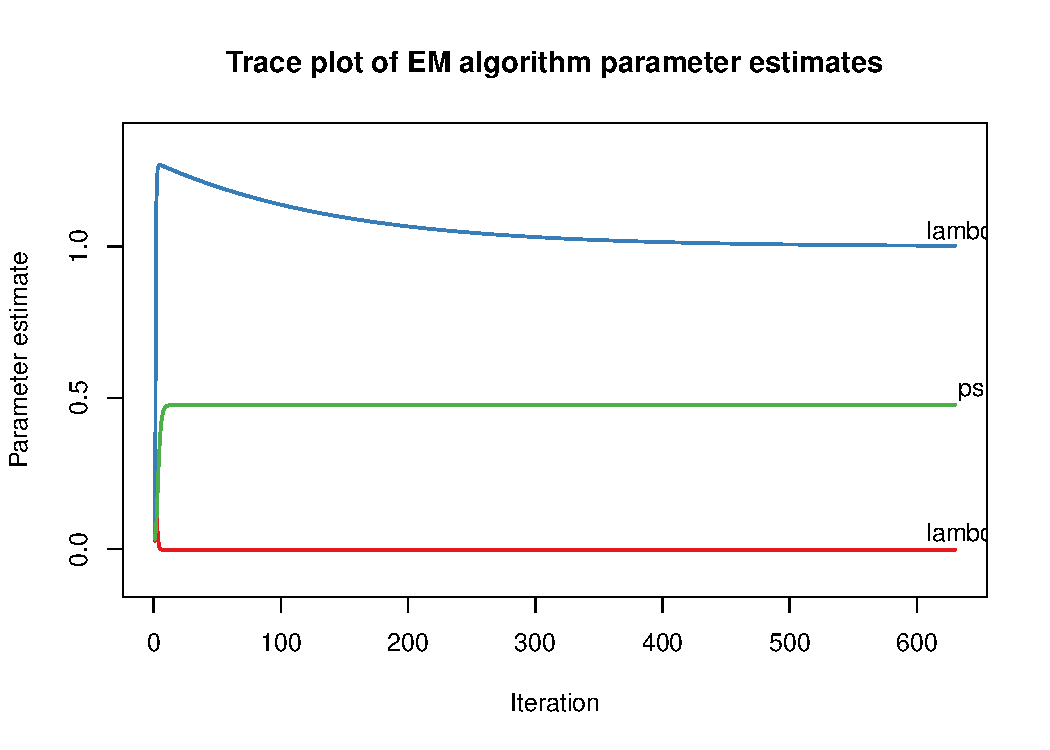
\includegraphics[width=12cm,height=7.6cm]{figure/syntax_progplot-1} 

}



\end{knitrout}

\item \code{report}

This controls the rate of reporting by the \code{iprior()} function. Defaults to every \code{report = 100} iterations.

\item \code{lambda, psi, sigma}

These are options to set the initial values of the parameters. For convenience, the user may choose to input one of \code{psi} or \code{sigma}, but not both, since \verb@psi = 1 / sigma ^ 2@.

\end{enumerate}

%\end{document}
